\documentclass[11pt]{m2pi}
%%%%%%%%%%%%%%%%%%%%%%%%%%%%%%%%%%%%%%%%%%%%%%%%%%%%%%%%%%%%%%%%%%%%%%
%                          STANDARD PACKAGES                         %
%%%%%%%%%%%%%%%%%%%%%%%%%%%%%%%%%%%%%%%%%%%%%%%%%%%%%%%%%%%%%%%%%%%%%%

\usepackage{graphicx}
\graphicspath{{figures/}}

\usepackage{epstopdf}
\usepackage{amsthm}
\usepackage{amsmath}
\usepackage{amssymb}
\usepackage{amsxtra}
\usepackage{amscd}
\usepackage{verbatim}
\usepackage{rotating}
\usepackage{multirow}
\usepackage{multicol}
\usepackage{url}
\usepackage[margin=1.5in]{geometry}
\usepackage[all]{xy}

%%%%%%%%%%%%%%%%%%%%%%%%%%%%%%%%%%%%%%%%%%%%%%%%%%%%%%%%%%%%%%%%%%%%%%
%                        STANDARD ENVIRONMENTS                       %
%%%%%%%%%%%%%%%%%%%%%%%%%%%%%%%%%%%%%%%%%%%%%%%%%%%%%%%%%%%%%%%%%%%%%%

% Theorems

%Commented out this theorem style I  have no idea why it's even here - Erik
%\theoremstyle{theorem}
\newtheorem{theorem}{Theorem}[section]
\newtheorem{alphtheorem}{Theorem}
\renewcommand{\thealphtheorem}{\Alph{alphtheorem}}
\newtheorem{lemma}[theorem]{Lemma}
\newtheorem{corollary}[theorem]{Corollary}
\newtheorem{guess}[theorem]{Conjecture}
\newtheorem{definition}[theorem]{Definition}
\newtheorem{facts}[theorem]{Facts}
\newtheorem{proposition}[theorem]{Proposition}
\newtheorem{problem}[theorem]{Problem}
%\newtheorem{algorithm}[theorem]{Algorithm}
%\newtheorem{claim}{Claim}[theorem]
\newtheorem{claim}[theorem]{Claim}
\newtheorem{subclaim}{Claim}[theorem]
\renewcommand{\thesubclaim}{\thetheorem.\alph{subclaim}}
\newtheorem{example}[theorem]{Example}
%\newtheorem*{example*}{Example}
\newtheorem{result}[theorem]{Result}
\newtheorem{observation}[theorem]{Observation}
\newtheorem{numconjecture}[theorem]{Conjecture}

\newtheoremstyle{myexample}{3pt}{3pt}{}{}{\bfseries}{.}{ }{\thmname{#1}\thmnumber{ #2}\thmnote{ (#3)}}
\theoremstyle{myexample}
\newtheorem{numremark}[theorem]{Remark}

\newtheoremstyle{myremark}{3pt}{3pt}{}{}{\bfseries}{.}{ }{\thmname{#1}\thmnote{ (#3)}}
\theoremstyle{myremark}
\newtheorem{remark}{Remark}
\newtheorem*{remark*}{Remark}
\newtheorem*{remarks*}{Remarks}
\newtheorem*{observation*}{Observation}
\newtheorem*{example*}{Example}

\newtheoremstyle{conjecture}{3pt}{3pt}{\itshape}{}{\bfseries}{.}{ }{\thmname{#1}\thmnote{ (#3)}}
%\newtheoremstyle{conjecture}{3pt}{3pt}{\rmfamily}{}{\itshape}{.}{ }{\thmname{#1}}
\theoremstyle{conjecture}
\newtheorem{question}{Question}
\newtheorem*{question*}{Question}
\newtheorem{conjecture}{Conjecture}
\newtheorem{theorem*}{Theorem}


\numberwithin{equation}{section}

% References
\newcommand{\genericref}[2]{#1~\ref{#2}}
\newcommand{\generictworef}[3]{#1~\ref{#2} and \ref{#3}}
\newcommand{\genericthreeref}[4]{#1~\ref{#2}, \ref{#3} and \ref{#4}}
\newcommand{\thmref}[1]{\genericref{Theorem}{#1}}
\newcommand{\lemmaref}[1]{\genericref{Lemma}{#1}}
\newcommand{\claimref}[1]{\genericref{Claim}{#1}}
\newcommand{\remarkref}[1]{\genericref{Remark}{#1}}
\newcommand{\conjref}[1]{\genericref{Conjecture}{#1}}
\newcommand{\tableref}[1]{\genericref{Table}{#1}}
\newcommand{\figref}[1]{\genericref{Figure}{#1}}
\newcommand{\twofigref}[2]{\generictworef{Figures}{#1}{#2}}
\newcommand{\threefigref}[3]{\genericthreeref{Figures}{#1}{#2}{#3}}
\newcommand{\propref}[1]{\genericref{Proposition}{#1}}
\newcommand{\twopropref}[2]{\generictworef{Propositions}{#1}{#2}}

% Case environment
\newenvironment{genericcase}[6]{\medskip\par\noindent \csname#1\endcsname{#2 #3}#4 \csname#5\endcsname{#6}.\begin{indentation}{1.5em}{0em}\noindent\ignorespaces}{\end{indentation}}
\newenvironment{case}[2]{\noindent \textit{Case #1}: #2.\begin{indentation}{1.5em}{0em}}{\end{indentation}}

%Note that I changed  \textit{Subcase #1}. #2. to  \textit{Subcase #1}: #2.
%Erik

\newenvironment{subcase}[2]{\noindent \textit{Subcase #1}: #2.\begin{indentation}{1.5em}{0em}}{\end{indentation}}
\newenvironment{ulindent}[1]{\noindent \underline{#1:}\begin{indentation}{1.5em}{0em}\setlength{\parindent}{0em}}{\end{indentation}}
\newenvironment{bfcase}[1]{\par\medskip\begin{indentation}{1.5em}{0em}\noindent\hspace*{-1.5em}\textbf{#1:}}{\end{indentation}}
\newenvironment{itcase}[1]{\par\medskip\begin{indentation}{1.5em}{0em}\noindent\hspace*{-1.5em}\textit{#1:}}{\end{indentation}}
%\newcommand{\case}[2]{\noindent \textbf{Case #1}: #2:}

% Induction environment
\newenvironment{basecase}[1]{\noindent \textsc{Base case}: #1:\begin{indentation}{1.5em}{0em}}{\end{indentation}}
\newenvironment{inductionstep}[1]{\noindent \textsc{Induction step}: #1:\begin{indentation}{1.5em}{0em}}{\end{indentation}}

% Algorithm headers
\newcounter{algorithm}
\setcounter{algorithm}{0}
\renewcommand{\thealgorithm}{\thesection.\arabic{algorithm}}
\newenvironment{algorithm}[1]{%
  \null
  \refstepcounter{algorithm}%
  \hrule%
  \vspace{0.2em}%
  \noindent\textbf{Algorithm \thealgorithm} #1
  \vspace{0.2em}%
  \hrule%
  \vspace{0.2em}
  }{%
  \vspace{0.2em}%
  \hrule%
  \null
}

%%%%%%%%%%%%%%%%%%%%%%%%%%%%%%%%%%%%%%%%%%%%%%%%%%%%%%%%%%%%%%%%%%%%%%
%                          STANDARD COMMANDS                         %
%%%%%%%%%%%%%%%%%%%%%%%%%%%%%%%%%%%%%%%%%%%%%%%%%%%%%%%%%%%%%%%%%%%%%%

\newcommand{\ie}{i.e.}
\newcommand{\eg}{e.g.} 
\newcommand{\resp}{\emph{resp.\@\ }} 
\newcommand{\etal}{et~al.} 
\newcommand{\cf}{cf.}

\newcommand{\mathbif}[1]{\mathbf{\emph{#1}}}
\newcommand{\nth}[1]{\ensuremath{#1^{\textrm{th}}}}
\newcommand{\nrd}[1]{\ensuremath{#1^{\textrm{rd}}}}
\newcommand{\nst}[1]{\ensuremath{#1^{\textrm{st}}}}
\newcommand{\jth}{\nth{j}}
\newcommand{\kth}{\nth{k}}
\newcommand{\qth}{\nth{q}}
\newcommand{\rth}{\nth{r}}

\newcommand{\vfrac}[2]{\ensuremath{{}^{\displaystyle#1} \diagup {}_{\displaystyle#2}}}

\renewcommand{\pmod}[1]{\ \left({\rm mod\ } #1 \right)}

%%%%%%%%%%%%%%%%%%%%%%%%%%%%%%%%%%%%%%%%%%%%%%%%%%%%%%%%%%%%%%%%%%%%%%
%                      SAVING THEOREM NUMBERS                        %
%%%%%%%%%%%%%%%%%%%%%%%%%%%%%%%%%%%%%%%%%%%%%%%%%%%%%%%%%%%%%%%%%%%%%%

%\newcounter{temp}
%\def\savecounter#1{\newcounter{#1}\setcounter{#1}{\value{theorem}}}
%\def\changetheoremcounter#1{\setcounter{temp}{\value{theorem}}\setcounter{theorem}{\value{#1}}}%\csname the#1\endcsname}}
%\def\restoretheoremcounter{\setcounter{theorem}{\value{temp}}}

\newcounter{temp}
\newcounter{ctemp}
\def\savecounter#1#2{%
   \newcounter{#1}%
   \setcounter{#1}{\value{section}}%
   \newcounter{#2}\setcounter{#2}{\value{theorem}}}
\def\swapcounter#1#2{%
   \setcounter{ctemp}{\value{section}}%
   \setcounter{section}{\value{#1}}%
   \setcounter{temp}{\value{theorem}}%
   \setcounter{theorem}{\value{#2}}%
   \addtocounter{theorem}{-1}}
\def\restorecounter{%
   \setcounter{section}{\thectemp}%
   \setcounter{theorem}{\thetemp}}

% \newcommand --------------------------------------------------------------
\newcommand{\eps}{\varepsilon}
\newcommand{\vf}{\varphi}
\newcommand{\cP}{\mathcal{P}}
\newcommand{\cH}{\mathcal{H}}
\newcommand{\cL}{\mathcal{L}}
\newcommand{\cM}{\mathcal{M}}
\newcommand{\cB}{\mathcal{B}}
\newcommand{\cD}{\mathcal{D}}
\newcommand{\cF}{\mathcal{F}}
\newcommand{\cO}{\mathcal{O}}
\newcommand{\cS}{\mathcal{S}}
\newcommand{\cN}{\mathcal{N}}
\newcommand{\cT}{\mathcal{T}}
\newcommand{\cU}{\mathcal{U}}
\newcommand{\fD}{\mathfrak{D}}
\newcommand{\fX}{\mathfrak{X}}
\newcommand{\fS}{\mathfrak{S}}
\newcommand{\bF}{\mathbb{F}}
\newcommand{\bH}{\mathbb{H}}
\newcommand{\bP}{\mathbb{P}}
\newcommand{\bR}{\mathbb{R}}
\newcommand{\bN}{\mathbb{N}}
\newcommand{\bS}{\mathbb{S}}
\newcommand{\bL}{\mathbb{L}}
\newcommand{\sF}{\mathscr{F}}
\newcommand{\sJ}{\mathscr{J}}
\newcommand{\sL}{\mathscr{L}}
\newcommand{\sS}{\mathscr{S}}
\newcommand{\sB}{\mathscr{B}}
\newcommand{\sA}{\mathscr{A}}
\newcommand{\sH}{\mathscr{H}}
\newcommand{\sP}{\mathscr{P}}
\newcommand{\la}{\langle}
\newcommand{\ra}{\rangle}
\newcommand{\intl}{\interleave}
\newcommand{\rrow}{\rightarrow}
\newcommand{\tbf}{\textbf}
\newcommand{\ves}{\varepsilon}

\begin{document}

\title{Modelling Canadian heavy crude congestion pricing}

\author{Wenning Wei}
\address{University of Calgary, Dept. of Math. and Stat.
2500 University Drive NW, Calgary AB, T2N 1N4, Canada}
\email{wenning.wei@ucalgary.ca}

\author{Erik Chan}
\address{University of Calgary, Dept. of Math. and Stat.
2500 University Drive NW, Calgary AB, T2N 1N4, Canada}
\email{erik.chan@ucalgary.ca}


%%%%%%%%%%%%%%%%%% FILL THIS IN %%%%%%%%%%%%%%%%%%%%%%%%%%%%%%%%
\author{Mahsa Azizi}
\address{}
\email{}

\author{Xilai Fu}
\address{}
\email{}

\author{Parisa Torabi}
\address{}
\email{}

%%%%%%%%%%%%%%%%%% FILL THIS IN %%%%%%%%%%%%%%%%%%%%%%%%%%%

\thanks{Acknowledge PIMS, any other funding sources (NSERC etc) here.}

\begin{abstract}
Insert abstract
\end{abstract}


\maketitle

\section{Introduction and Motivation}
Spatial price integration in oil commodity markets is a topic of interest to evaluate the degree of oil price integration between different geographic locations world wide. Depending on the oil type, light or heavy, the price that a producer receives for a barrel of oil varies. In addition  \cite{Zhu2020}



\section{Model}
Using the surcharge estimation model (SEM) in \cite{Zhu2020}, we have the following mixed-integer and linear programming 
\begin{equation}\label{1}
\begin{split}
\text{minimize: } &\sum_{s\in\cS} \alpha_s\\
\text{subject to: } &\lambda_s^t = \rho_s + \ves_s^t +\omega_s^t, \quad \forall s\in\cS,~\forall t\in\cT,\\
&-\alpha_s\leq\ves_s^t \leq \alpha_s,\\
&0\leq\omega_s^t\leq \psi^t M,\\
&\ves_s^t \geq \alpha_s - (1-\gamma_s^t) M,\\
&\sum_s \gamma_s^t\geq \psi^t,\\
&\sum_t \psi^t \leq \beta M,\\
&\psi^t, \gamma_s^t \in\{0,1\},
\end{split}
\end{equation}
where $\lambda_{s}^{t}$ is the price spread of customer node $s$ and producer, M is a number big enough, $\beta\in[0,1]$ is a predetermined parameter representing the proportion of the time period that the surcharge term $\omega_s^t$ can take positive value.

When there is only one customer node, the above programming problem reduces to
\begin{equation}\label{2}
\begin{split}
\text{minimize: } &\alpha\\
\text{subject to: } &\lambda^t = \rho + \ves^t +\omega^t, \quad \forall t\in\cT,\\
&-\alpha\leq\ves^t \leq \alpha,\\
&0\leq\omega^t\leq \psi^t M,\\
&\ves^t \geq \alpha - (1-\psi^t) M,\\
&\sum_t \psi^t \leq \beta M,\\
&\psi^t \in\{0,1\}.
\end{split}
\end{equation}


\section{Result}
We take Hardisty as the producer node with WCS as the price, and Cushing the customer node with WTI-5 as the price, with \$5/bbl as the heavy/light spread. Here there is only one customer node. Using the programming problem \eqref{2}, we get the following result.

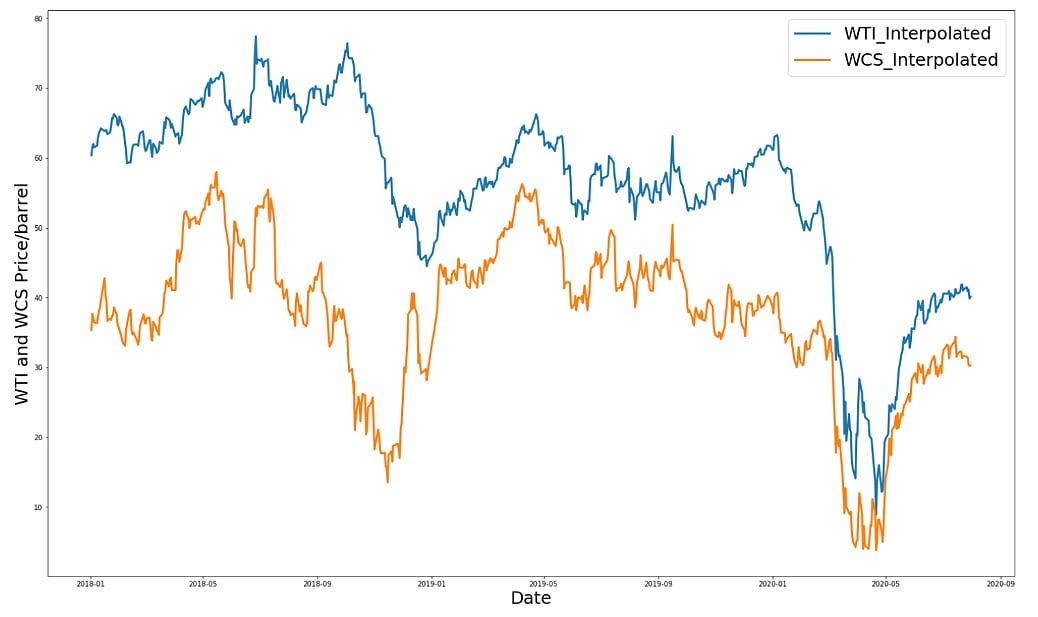
\includegraphics[height=3in, width= 6in]{WTI-WCS-Price.PNG}

With the data of WCS and WTI during the time interval Jan. 2018 to Jul. 2020, we get the following result for different value of $\beta$.

\includegraphics[height=2in, width= 6in]{beta0.2}

\includegraphics[height=2in, width= 6in]{beta0.4}

\includegraphics[height=2in, width= 6in]{beta0.6}

\includegraphics[height=2in, width= 6in]{beta0.8}

\section{Documented disruption}
From January to July 2018, in western Canada, production increased steadily while export capacity remained at 2016 levels or below leading to large price discounts for Canadian crude benchmarks. As a result, WCS has averaged US\$21.86 lower than WTI, an increase in the differential of 71\% over the same period in 2017. While some discount should be expected based on quality and transportation costs to American refineries compared to other light crude streams, this normally ranges between US\$10 and US\$15. Western Canadian heavy oil production increased by 9.8\% in 2017, and in the first half of 2018 was 8\% higher year-over-year. Without incremental pipeline capacity available, some production has shifted to rail, which is more expensive.~\cite{bibid} {\color{red} What is cite\{bibid\} ??} 

In fall 2018, the WCS--WTI differential widened further than normal. This means that Canada received a much lower price for its oil than normal and many market participants were negatively affected. The primary factor behind these wide oil price differentials was a growing supply of western Canadian oil production to 4.30 million barrels per day (b/d) in September 2018. Takeaway capacity on existing pipeline systems remained constant at around 3.95 million b/d. In addition, refinery maintenance in the United States (U.S.) Midwest, the largest export market for Canadian heavy crude oil, led to a significant reduction in demand for Canadian oil.~\cite{bibid} {\color{red} What is cite\{bibid\} ??} 
\section{Network with a pseudo location}
Model the spread as an OU process
\[dx_t  = \alpha(\mu-x_t)\,dt + \sigma dW_t\]
By the maximum log-likelihood, we get the following parameters:  $\alpha=0.0118$,$\mu=16.275$, $\sigma=2.053$.
We use a simulated process as the spread of WCS and the price at the pseudo location

%\includegraphics[height=2in, width= 6in]{simulatedpath}

Using the programming problem \eqref{1} with two consumer nodes Cushing and the pseudo location, we get the following result.

\section{Acknowledgements}
Thank people here.

\bibliographystyle{amsplain}
\bibliography{project}

\end{document}
